\section {Literature research}
\chapterauthor{Agnieszka Kuleta}
\subsection{Needs for specific diet growing}
In recent years, there has been a notable increase in people following specific diets\cite{martin2020prescription}.  For some, dietary restrictions are necessary to manage health issues or food sensitivities, while others adopt these diets to lose weight, build muscle, or reduce their environmental impact.
\par
They are various reasons why we as a population decide to take the effort of being on diet. According to \textbf{US National Center for Health Statistics}\cite{martin2020prescription} this need increased with increasing each person obesity index and increasing educational level. Whats why Americans participating in study  usually have chosen diets connected to weight loss. They were choosing mostly low carbohydrate or low calories diets. Their aim was really simple to loss weight. However, for younger generations this is not enough, now GEN Z is taking step forward \cite{haddon2024genz}. They are introducing the training and healthy eating as a lifestyle. They love to lift weights and eat proteins \cite{fortune2024gym}. For them our portal would be also very helpful as  we marked it in the Persona model which will be fully presented in \textit{"Requirements"} chapter. Let's say that it will be our first cause that provides the need of diets.
\par
The second, and for us the most important, reason for creating this app is to support people who must follow specific diets due to food allergies. According to \textbf{World Health Organization} \cite{whoAllergy}, globally more than 220 million people are forced to avoid certain foods because of allergies. There are really limited protection of individuals with food allergies because the only solution is to strictly adhere to restrictions. The serious health risks done by allergens and the limited treatment options available highlight the importance of knowing which foods are most commonly associated with severe allergic reactions. Moreover, according to online side \textbf{Food Allergy Research and Education}\cite{foodallergy} having a food allergy heavily impacts the quality of life, not only the person who has it, but also their relatives. The disease results in exclusion of children from school canteens and prevents their full participation in school life and society. It also is written that, mothers of food-allergic children under age five have significantly higher blood-pressure measurements than mothers whose children do not have food allergies. That is also why we took one mum as a Persona model which will be fully presented in \textit{"Requirements"} chapter. That mum does not know how to deal with food allergy of her child and needs application to gain the ideas of new recipes. Mum also tries to cook for a whole family as close to "normally" as possible, without the constant worry of accidental exposure to allergens. That's why in our application we will take into account gluten-free and no-dairy diets, because they are two most common and the hardest to avoid allergens on the daily basis.
\par
Finally, the last but not least reason why people want to change the way of eating are health, environment and morality \cite{WhyVegan}. After a  quick glance at the websites \cite{WhyVegan} of  vegan and vegetarian organizations gives three  mentioned reasons are the answer to the question why people do adopt a plant-based lifestyle. This shift is more than a dietary change; it represents a comprehensive transformation in mindset. The approach to meat consumption among vegans and vegetarians shows minimal difference during the initial stages, as illustrated on Figure\ref{fig:Why people become vegan and vegetarians}.
  
\begin{figure}[ht]
    \centering
    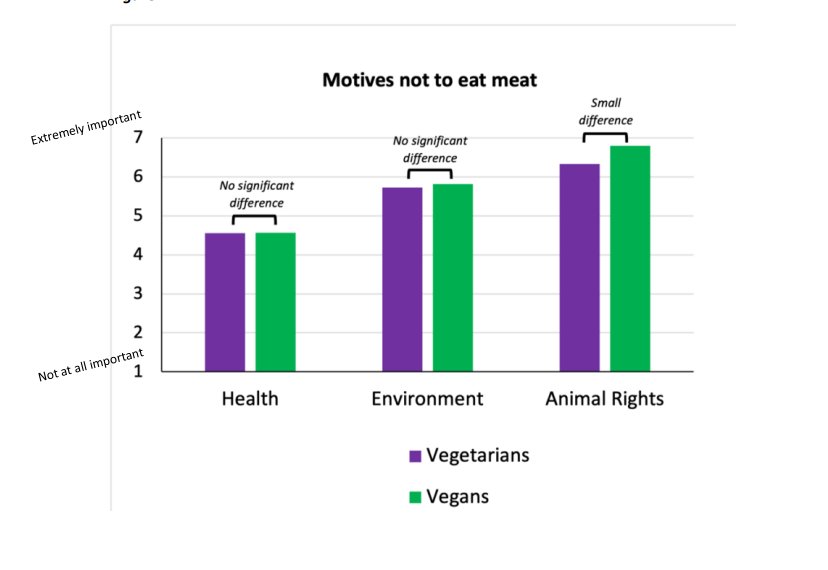
\includegraphics[width=0.8\textwidth]{images/vv.png}
    \caption{Motives not to eat meat vegans vs vegetarians \cite{2021Vegan}.}
    \label{fig:Why people become vegan and vegetarians}
\end{figure}

From the chart we might see that people who are vegan and vegetarians similarly value Health and Environment factors. However, animal rights show a difference. They are more important to vegans than to vegetarians.
Such a distinction suggests that while both diets are plant-based, the motivation behind a vegan lifestyle may lead to stricter dietary choices focused on minimizing harm to animals.
\par
For each diet we would like to give you quick overview by highlighting what should be eat and what should be avoided. Of course, we are fully aware that we will not describe and mark every existing diet, we just want to give you the main idea of each diet included in our application. To make it far easier and faster to get to know strict rules and restriction for each diet without any details and insights, we have prepared Table \ref{tab:all_diets_overview}.

\begin{table}[H]
\resizebox{\columnwidth}{!}{%
\begin{tabular}{|c|c|c|c|c|c|c|}
\hline
           & VEGAN & VEGETARIAN & OMNIVORE & LACTOSE -ALLERGIC & GLUTEN-ALLERGIC & KETO \\ \hline
MEAT       &       &            & X        & X                 & X               & X    \\ \hline
EGGS       &       & X          & X        & X                 & X               & X    \\ \hline
WHEAT AND OATS      & X     & X          & X        & X                 &                 & X    \\ \hline
DAIRY      &       & X          & X        &                   & X               & X    \\ \hline
VEGETABLES & X     & X          & X        & X                 & X               &      \\ \hline
FRUITS     & X     & X          & X        & X                 & X               &      \\ \hline
SOY       & X     & X          & X        & X                 & X               & X    \\ \hline
PEANUTS    & X     & X          & X        & X                 & X               & X    \\ \hline
\end{tabular}%
}
\caption{Products categories included in each diet}
\label{tab:all_diets_overview}
\end{table}
 
\subsubsection{Obesity and fit trend reason}
While contemporary fitness and weight management trends often prioritize calorie counting and macro-elements tracking, there is less focus on the diversity of food. To follow these type of diets the key is calories counting and nutrition elements counting. 
\begin{itemize}
    \item \textbf{Low calories}  \newline
    The main idea of this diet is too feel full on fewer calories. Achieving this goal often requires meticulous calorie counting for each meal. Tracking calorie intake helps ensure you stay within a set daily limit and allows for better planning of subsequent meals to meet those goals. According to the Mayo Clinic \cite{lowcalories}, choosing the low-calories diet for most adults typically reduces daily intake to between 1,200 and 1,800 calories, though this range may be too restrictive for some, depending on their health status and history. Rather than focusing on specific foods to eat or avoid, the key is consistently sticking to your daily calorie limit.\newline
    \item \textbf{Ketogenic diet}  \newline
    A ketogenic diet is a low-carbohydrate, high-fat diet,  focuses on drastically reducing carbohydrate intake while increasing fats to put the body into a state called ketosis. In ketosis, the body burns fat for energy instead of carbs. In order to trigger ketosis, the carbs you eat need to be heavily restricted – down to no more than 20-50 grams per day. According to \textbf{Health direct in Australia } \cite{keto1}, it is proved that it works for long term weight lost. However not everyone can use it for example it is really bad for children. The main goal of this diet is to reduce carbs.  So the main foods which is included a ketogenic diet are high quality fats like: 
    \begin{itemize}
        \item avocado 
        \item olive oil 
        \item coconut oil 
        \item nuts and seeds
    \end{itemize}
    Also, every kind of meat or fish source and eggs, which is not only full of fats but also proteins. You may have some low carbohydrate vegetables, such as lettuce and cucumbers. On a typical ketogenic diet, you will have only small amounts of rice, pasta, fruit, grains, bread, beans and starchy vegetables such as peas and potatoes, because all of these ingredients are full of carbs. And of course, you should not eat: fruits, preprocessed sweets and snacks like chips, drinking alcohol, sugar. In the Table \ref{tab:keto}, it is establish which products are worth eliminating and what can be eaten in exchange \cite{ketotable1} \cite{ketotab2}. 
        \begin{table}[H]
            \centering
            \scriptsize
            \renewcommand{\arraystretch}{1.3}
            \begin{tabular}{|c|c|}
            \hline
            \textbf{To Eliminate} & \textbf{Substitute} \\ \hline
            Wheat & Almond flour, Coconut flour \\ \hline
            Rice & Cauliflower rice, Shirataki rice \\ \hline
            Sugar & Erythritol, Stevia, Monk fruit, Allulose \\ \hline
            Bananas & Strawberries \\ \hline
            Apples & Raspberries \\ \hline
            Oranges & Blackberries \\ \hline
            Butter & Avocado \\ \hline
            Pasta & Zucchini noodles \\ \hline
            \end{tabular}
            \caption{Keto diet ingredients to eliminate and their substitutes}
            \label{tab:keto}
        \end{table}
\end{itemize}

\subsubsection{Allergenic reasons}
Firstly, we might wonder why allergies are so frustrating - why they are reasons to limit ourselves? An allergy is a health response triggered by a specific immune reaction to certain foods. These dietary restrictions are increasingly common, driven by the rising number of food allergies. But what foods commonly cause these reactions? Would not it be simpler if only a single ingredient were to blame?
\par
According to U.S. Department of Agriculture \cite{allergybig9}, allergic reactions might be caused by more than 160 foods, however there are 9 most common items established by them, which account for 90 percent of food allergic reactions. There are called BIG9:
\begin{itemize}
    \item milk
    \item eggs
    \item fish
    \item shellfish
    \item tree nuts
    \item peanuts
    \item wheat
    \item soybeans 
    \item sesame
\end{itemize}

Each restriction differ and it is not easy to deal with any of it. However, taking for an example wheat and peanuts what would be easier for you to eliminate? Or wheat and eggs? What do you choose? Now, imagine being unable to consume either lactose or gluten. What could you eat then? Would you have to rely solely on a vegan, gluten-free diet? 
In this chapter, we will focus on gluten-free and dairy-free diets, as they pose some of the greatest challenges due to the widespread presence of these ingredients in typical European meals. 

\subsubsection{Gluten-free diet}
First question crossing our mind is what exactly gluten is? According to \textbf{Celiac Disease Foundation}\cite{WhatIsGluten} is a type of protein found in grains such as wheat, barley, rye and oats. Sensitivity to gluten is a symptom of three main disorders: celiac disease, wheat allergy, and non-celiac gluten sensitivity. All of these illnesses have common symptoms like diarrhea, stomach pain, and vomiting. 
Unfortunately, the only way  to improve health and avoid all the symptoms is making careful dietary choices and avoid foods made from gluten-containing grains. But what type of food contains it?
Unfortunately we have quite big amount of food to avoid to:
breads, pastas/noodles, cereals, dumplings, soy sauce, fried/breaded foods, pastries, cake, crusts, cookies, crackers, tortillas, gravy/thick sauces, beer. And now let's see how do we can substitute it?
The answer to this question can be found in the Table \ref{tab:gluten}. This table was prepared based on blogs \cite{GlutenFreeDiet}\cite{GlutenFreeSubstitutions}\cite{ActivateGlutenFree} and own experiences.

\begin{table}[H]
\centering
\scriptsize
\begin{tabular}{|c|c|}
\hline
\textbf{TO ELIMINATE} & \textbf{SUBSTITUTE} \\ \hline
COUSCOUS                     & CAULIFLOWER             \\ \hline
CORNSTARCH                  & ARROWROOT               \\ \hline
OATS                         & GLUTEN FREE  OATS       \\ \hline
BREAD CRUMBS                 & ALMOND MEAL             \\ \hline
PASTA                        & ZUCCHINI, CHICKPEA PASTA, QUINOA PASTA, CORN PASTA \\ \hline
LOLLIES                      & NUTS                    \\ \hline
SOY SAUCE                    & TAMARI SAUCE            \\ \hline
MALT VINEGAR                 & BALSAMIC VINEGAR        \\ \hline
NOODLES                      & SHIRATAKI NOODLES, RICE NOODLES      \\ \hline
CEREALS                      & GLUTEN-FREE CEREALS     \\ \hline
SOY SAUCE                    & COCONUT AMINOS, TAMARI SAUCE         \\ \hline
BREADCRUMBS                  & CRUSHED CORNFLAKES, RICE CRACKERS, GLUTEN-FREE BREADCRUMBS \\ \hline
TORTILLAS                    & CORN TORTILLAS          \\ \hline
BEER                         & HARD CIDER              \\ \hline
FLOUR                        & COCONUT FLOUR, RICE FLOUR, ALMOND FLOUR \\ \hline
BULGUR                       & RICE, BUCKWHEAT, QUINOA\\ \hline
COUSCOUS                     & QUINOA                  \\ \hline
FARINA                       & CREAM OF RICE           \\ \hline
GRAHAM FLOUR                 & ALMOND FLOUR            \\ \hline
HYDROLYZED VEGETABLE PROTEIN & SOY PROTEIN ISOLATE     \\ \hline
SEITAN                       & TEMPEH, JACKFRUIT, TOFU \\ \hline
WHEAT BERRIES                & QUINOA, BROWN RICE      \\ \hline
WHEAT GERM                   & CHIA SEEDS              \\ \hline
MALT                         & BROWN RICE SYRUP        \\ \hline
BROWN RICE SYRUP             & MAPLE SYRUP, HONEY       \\ \hline

\end{tabular}
\caption{Gluten-free diet forbidden products and their substitutes}
\label{tab:gluten}
\end{table}

\subsubsection{Dairy-free diet}
Typical European diet contains  yogurt, butter or cheese made from the milk of animals including that from cows, goat or sheep. However, many people are unable digest the lactose in milk. According to \textbf{Arizona Digestive Health} \cite{ArizonaDigestive2024Lactose}, it is estimated that approximately 65 percent of the world’s population is lactose intolerant. However, it is only one from may reasons, people also can have milk-allergy. For these people eating products which contain lactose cause the allergic reaction by causing symptoms like discomfort, stomach pain and  diarrhea. There are no other cure than diet. So these people have to follow restrictions of the diet, which is avoiding lactose-a type of simple sugar found naturally in milk.
This type of diet avoids all milk-derived ingredients, including obvious ones like cheese, butter, cream, and yogurt, as well as less obvious sources such as whey, casein, and certain baked goods.
To successfully maintain a dairy-free diet, let's have a look at the Table \ref{tab:dairyfree}. This table was prepared based on blogs \cite{BBCDairyFree}\cite{HealthLactoseFreeDiet} and own experiences.

\begin{table}[H]
\centering
\scriptsize
\begin{tabular}{|c|c|}
\hline
\textbf{TO ELIMINATE} & \textbf{SUBSTITUTE} \\ \hline
Acid Casein       & Soy protein isolate, pea protein isolate                    \\ \hline
Cheese            & Dairy-free cheese slices (e.g., made from coconut oil, soy) \\ \hline
Asiago            & Cashew cheese                                               \\ \hline
Brie              & Cashew                                                      \\ \hline
Butter            & coconut                                                     \\ \hline
Butter Oil        & Coconut oil                                                 \\ \hline
Buttermilk        & apple cider vinegar                                         \\ \hline
Camembert         & Cashew                                                      \\ \hline
Caramel           & Coconut milk caramel                                        \\ \hline
Condensed Milk    & soy milk                                                    \\ \hline
Cream             & Coconut cream, oat cream, or cashew cream                   \\ \hline
Feta              & Tofu feta, almond-based feta                                \\ \hline
Fontina Cheese    & Plant-based cheese with a mild flavor (e.g., cashew cheese) \\ \hline
Gorgonzola        & Marinated tofu                                              \\ \hline
Kefir             & Coconut kefir                                               \\ \hline
Low Fat Milk      & Almond milk, oat milk, or soy milk                          \\ \hline
Ricotta           & Almond ricotta, tofu ricotta, or cashew ricotta             \\ \hline
Yogurt            & Coconut yogurt, almond yogurt, soy yogurt                   \\ \hline
Whole Milk Solids & Coconut milk powder, soy milk powder                        \\ \hline
Whey Peptides     & Pea peptides, rice protein peptides                         \\ \hline
\end{tabular}
\caption{Dairy-free diet forbidden products and their substitutes}
\label{tab:dairyfree}
\end{table}


\subsubsection{Environment and morality} 
Having said, why people usually switch to plant-base diet, let's have a look the differences between vegans and vegetarians.
According to study made by Kent University \cite{2021Vegan} more than 80 percent of studied population switched to vegan diet, because of  Animal ethics and comparing to vegetarians this reason is a little bit less popular. Between this two groups there is some disagreement as we can see on the Figure\ref{fig:vegansvsvegetarian}. 

\begin{figure}[H]
    \centering
    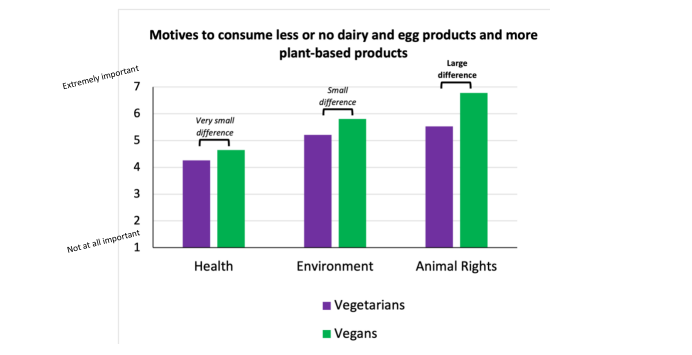
\includegraphics[width=0.8\textwidth]{images/vvsv.png}
    \caption{Differences between vegans and vegetarians approach\cite{2021Vegan}.}
    \label{fig:vegansvsvegetarian}
\end{figure}

This chart reflects not only psychological differences between this two groups but also explains the differences in diets. Explains why vegetarians only do not eat animals, but they eat the products which come from an animal, and vegans do not. The products, which are avoided by vegans and their substitutes, are in the Table \ref{tab:vegansub}. There are also marked in pink, products which are avoided by vegetarians too. 

\begin{table}[H]
\centering
\scriptsize
\begin{tabular}{|c|c|}
\hline
\textbf{TO ELIMINATE} & \textbf{SUBSTITUTE} \\ \hline
\rowcolor{purple!10} % Light green for alternating rows
Pig & Tofu, Seitan\\ \hline
\rowcolor{purple!10}
Beef & Tempeh, Jackfruit\\ \hline
\rowcolor{purple!10}
Chicken & Oyster mushrooms, Tofu \\ \hline
\rowcolor{purple!10}
Veal & Mushrooms \\ \hline
\rowcolor{purple!10}
Fish sticks & Vegan fish sticks \\ \hline
\rowcolor{purple!10}
Cod & Banana blossom \\ \hline
\rowcolor{purple!10}
Shrimps & Tofu \\ \hline
\rowcolor{purple!10}
Crabs & Hearts of palm \\ \hline
\rowcolor{purple!10}
Salmon & Artichoke, Seaweed \\ \hline
\rowcolor{purple!10}
Tuna & Soy watermelon \\ \hline
Milk                   & Rice milk, Coconut milk, Oat milk, Soy milk, Almond milk  \\ \hline

Cheese                 & Cashew cheese, Almond-based cheese, Soy cheese, Violife    \\ \hline
Butter                 & Avocado oil, Coconut oil                      \\ \hline
Yogurt                 & Oat-based/ Coconut-based /Soy-based /Almond-based yogurt    \\ \hline
Cream                  & Soy-based cream,Cashew cream                  \\ \hline
Eggs (scrambled)       & Chickpea flour scramble          \\ \hline
Eggs (baking)          & Chia seed, Applesauce             \\ \hline
Honey                  & Agave nectar, Date syrup, Brown rice syrup, Maple syrup   \\ \hline
Gelatin                & Carrageenan, Pectin, Agar-agar                      \\ \hline
Lard                   & Vegan margarine, Coconut oil, Vegetable shortening   \\ \hline
Carmine (red coloring) & Beet juice                       \\ \hline
Casein and Lactose     & Soy protein                      \\ \hline
Shellac                & Vegan-friendly coatings          \\ \hline

% Continue with other rows as needed
\end{tabular}
\caption{Plant-based Alternatives to Common Animal Products}
\label{tab:vegansub}
\end{table}

Having said about all diets, which were detailed analyzed and explained, it is time to focus on our main goal of the app. Our main requirement is to substitutes disliked products or allergens. So we have also done the research how we can substitute every ingredient in our app for different products. When we were choosing substitutes we were looking for thousands of blogs and we were testing some recipes at home to find the right substitutes, which were similar in texture and flavor to original products.

\section{Existing systems} 
\label{section:existing_solutions}
\chapterauthor{Agnieszka Kuleta}\newline
After discussing various diets and the motivations behind dietary restrictions, we did necessary overview to determine whether any existing applications align with our core ideas and concepts. Our main ideas and needs were outlined in the "Motivation" section, the complete system functionalities will be detailed in the "Requirements" chapter.
\par
Table \ref{tab:existing_solutions} highlights the functionalities of popular culinary platforms, especially familiar to Polish students. Our goal was to identify which platform, if any, could meet the requirements set by our stakeholders. Unfortunately, none of the reviewed platforms did so. It might be easily concluded by making comparative analysis presented in the table. This analysis highlights the uniqueness of our functionalities and the need to implement our solution.

Further details on the specific requirements and functionalities, design and implementation will be provided in the following chapters.


\renewcommand{\arraystretch}{1.5}
\begin{landscape}
\begin{table}[H]
\Large
\resizebox{\columnwidth}{!}{%
\begin{tabular}{lllll}
                                                                            & aniagotuje.pl & https://www.kwestiasmaku.com/ & https://www.jamieoliver.com/ & Foodies \\
LOG IN                                                                      & y             & y                             & y                            & y          \\
SAVING RECEPIES                                                             & y             & y                             & y                            & y          \\
ADDING NOTES                                                                & y             & y                             &                              &            \\
SEARCHING FOR RECIPIE                                                       & y             & y                             & y                            & y          \\
ADDING COMMENTS                                                             & y             & y                             &                              & y          \\
GIVING RATING                                                               & y             & y                             &                              & y          \\
CATEGORIES (LIKE DINNER, BREAKFAST)                                         & y             & y                             & y                            & y          \\
PRINTING OF RECEPIES                                                        & y             & y                             &                              &            \\
SELF CALCULATING MACROELEMENTS                                              &               &                               &                              & y          \\
GIVEN MACROELEMENTS                                                         & y             & y                             & y                            & y          \\
ADDING FOTO IN COMMENTS                                                     &               & y                             &                              & y          \\
NEWSLETTER SUBSCRIPTION                                                     & y             &                               & y                            &            \\
COOK MODE (KEEP SCREEN AWAKE)                                               & y             &                               &                              & y          \\
COPY ALL INGREDIENTS BY ONE CLICK                                           & y             &                               &                              &            \\
SORTING &
  publication date and popularity &
  \multicolumn{2}{l}{publication date and popularity} &
  by number of calories, by rating \\
TAGS                                                                        & y             &                               & y                            &            \\
FILTERS &
  \multicolumn{3}{l}{by diets : glutten free, vegan,   vegetarian} &
  by number of calories, by diets \\
DIETS &
  omnivore, glutenfree, vegan, vegaterian &
  omnivore, glutenfree, vegan, vegaterian &
  omnivore, glutenfree, vegan, vegaterian, diary free &
  omnivore, glutenfree, vegan, vegaterian, diary free, keto \\
MACROELEMNTS MORE DETAILED(NOT ONLY   CALORIES)                             & y             &                               & y                            & y          \\
POSIBILITY FOR EDITING USER'S DATA                                          &               & y                             &                              & y          \\
CULINARY CALCULATOR (IE. HOW MANY GRAMS   IS A SPOON)                       &               & y                             &                              &            \\
BACKING CALCULATOR (IE. HOW MANY SMALL   FRAMES TO USE INSTEAD OF BIG ONE)? &               & y                             &                              &            \\
DISLIKED INGREDIENTS LIST                                                   &               &                               &                              & y          \\
MODIFYING RECEPIES                                                          &               &                               &                              & y          \\
SAVING MODIFIED RECEPIES                                                    &               &                               &                              & y          \\
SUBSTITUTING INGREDIENTS IN RECIPIE                                         &               &                               &                              & y         
\end{tabular}%
}
\caption{Comparison of existng solutions}
\label{tab:existing_solutions}
\end{table}
\end{landscape}
